\section{Introducción}
\iffalse
Ejemplo enumeración:
\begin{enumerate}
	\item Item1
	\item Item2
\end{enumerate}
Aquí se referencia a la imagen \ref{prueba} y aquí a la imagen \ref{prueba_invertida}

Ejemplo figura:
\begin{figure}[h]
	\centering
	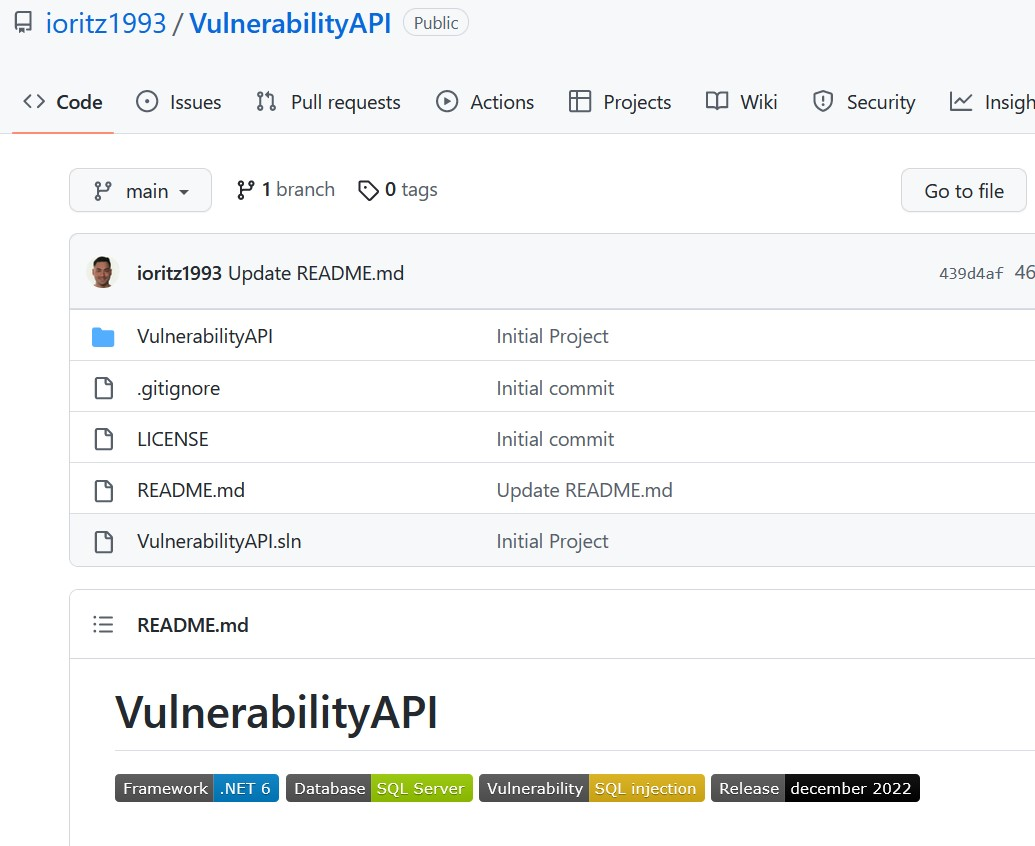
\includegraphics[width=160mm]{includes/ejemplo_figura.jpg}
	\caption[Ejemplo figura]{Ejemplo figura (Elaboración propia)}
	\label{prueba}
\end{figure} 

\begin{figure}[h]
	\centering
	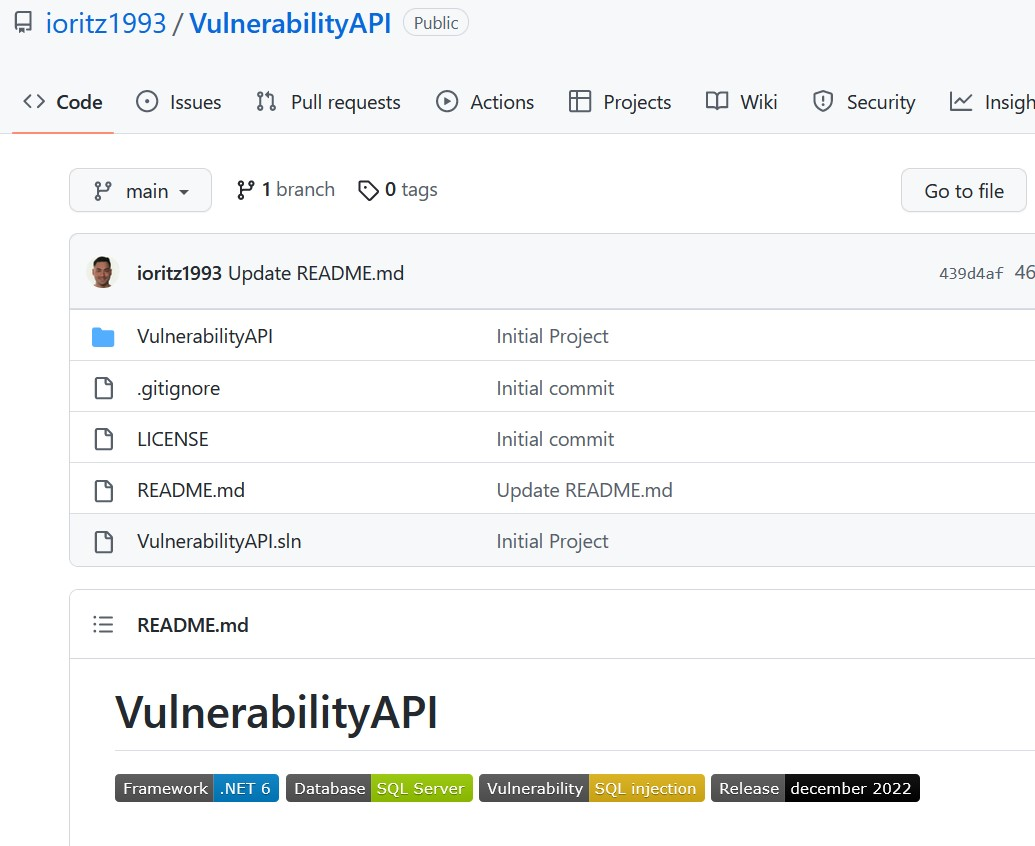
\includegraphics[width=160mm, angle=180]{includes/ejemplo_figura.jpg}
	\caption[Ejemplo figura girada]{Ejemplo figura girada (Elaboración propia)}
	\label{prueba_invertida}
\end{figure} 
\fi

La movilidad urbana eficiente se ha convertido en un reto prioritario para las administraciones públicas, especialmente en territorios con alta densidad poblacional y complejidad geográfica. La creciente demanda de desplazamientos, junto con la necesidad de garantizar la sostenibilidad del sistema de transporte, exige soluciones avanzadas que permitan optimizar el uso de las infraestructuras existentes y reducir los impactos negativos del tráfico. Una gestión adecuada del tráfico no solo repercute en la calidad de vida de la ciudadanía, sino que también incide directamente en la reducción del consumo energético, la mejora de la seguridad vial y la disminución de la contaminación atmosférica.

En la provincia de Bizkaia, estos desafíos se intensifican debido a varios factores estructurales y ambientales. Por un lado, su orografía accidentada limita la expansión de la red vial y concentra los flujos de tráfico en determinados corredores estratégicos. Por otro, la alta concentración urbana en el área metropolitana de Bilbao genera elevados niveles de congestión, especialmente en horas punta. Además, la variabilidad meteorológica, con episodios frecuentes de lluvia o niebla, puede alterar de forma significativa las condiciones de circulación, introduciendo incertidumbre en la gestión diaria del tráfico.

En este contexto, la predicción del tráfico emerge como una solución clave, al permitir estimar de forma anticipada el comportamiento del flujo vehicular a partir del análisis de datos históricos y condiciones externas. Durante los últimos años, el avance en el ámbito de la inteligencia artificial, y en particular del aprendizaje profundo, ha facilitado la creación de modelos cada vez más precisos para esta tarea. Entre las arquitecturas más prometedoras se encuentra la basada en Transformers, ampliamente reconocida por su capacidad para modelar dependencias a largo plazo y procesar grandes volúmenes de datos secuenciales con eficiencia.

Este trabajo tiene como objetivo el desarrollo de un modelo predictivo basado en Transformers, enfocado específicamente en el entorno de Bizkaia, y alimentado con datos abiertos de tráfico y meteorología publicados por organismos públicos. Se busca con ello generar una solución tecnológica que permita anticipar de manera fiable el estado del tráfico en distintas zonas del territorio y contribuir así a una gestión más inteligente, preventiva y sostenible de la movilidad urbana.

El trabajo se va a estructurar de la siguiente forma. Para comenzar, se va a contextualizar el problema y se van a definir los objetivos, detallando los retos del tráfico en Bizkaia y justificando la necesidad del modelo previsto. Posteriormente, se va a definir la metodología que se va a seguir. Seguidamente, se va a realizar el estudio del estado del arte, recogiendo las principales aproximaciones en cuanto a técnicas para la predicción del tráfico. A continuación, se abordará el desarrollo específico del modelo propuesto, incluyendo todas las fases implicadas en su diseño, entrenamiento y validación. Para finalizar, se presentarán distintas opciones en cuanto a trabajo futuro a llevar a cabo y se expondrán las conclusiones extraídas.

